% L15a the utility basket and betting against beta. Two panels on the same market sensitivity axis.
% Left: the factor 1/max(|beta_i|, beta_floor)^xi_t that the preference weight applies to the expected
% growth rate, for a falling market (xi_t = 1, red), a rising market (xi_t = -1, blue), and xi_t = 0
% (gray, dashed). The three cross at beta_i = 1, where the factor is 1. Right: the betting-against-beta
% weights before the trading limits for eight made-up stocks with beta_i = 0.4, 0.6, 0.8, 0.95, 1.1, 1.3,
% 1.5, 1.8, from weigh_bab in strategies/weighting/bab.jl: the half below the middle rank goes long and
% the half above it goes short, and each side is scaled to a market sensitivity of one.
%
% November 27, 2026: drawn in the style of the L13a schematics (schematic-style.tex).
% Scale: 2.6 cm per unit of beta_i; 0.9 cm per unit of the factor; 2.4 cm per unit of weight.
\documentclass[tikz,border=6pt]{standalone}
% Shared style for the L15a schematics, copied from L14a (November 19, 2026), \input by each Fig-L15a-*.tex.
% Copied from week-13/L13a/figs/jumphmm-diagram.tex (the week-12 schematic style): same fonts,
% ink, accent colors, boxes, and arrows, plus a monospace font for tool names and order
% statuses. The notebook SVG carries a dark palette added by theme_svg.py; every color here
% must be mapped there.
\usepackage[no-math]{fontspec}
\IfFontExistsTF{Arial}{\setsansfont{Arial}}{\setsansfont{TeX Gyre Heros}}
\renewcommand{\familydefault}{\sfdefault}
\IfFontExistsTF{Menlo}{\setmonofont[Scale=0.92]{Menlo}}{}
\usepackage{amsmath,amssymb}
\usetikzlibrary{arrows.meta,calc,positioning,decorations.pathreplacing}

\definecolor{vnink}{HTML}{202124}
\definecolor{gdblue}{HTML}{0091FF}
\definecolor{gdred}{HTML}{E02020}
\definecolor{gdgray}{HTML}{6D7278}
\definecolor{saorange}{HTML}{F08C00}
\definecolor{boxfill}{HTML}{F1F3F4}
\definecolor{orangefill}{HTML}{FFE8C7}
\definecolor{bluefill}{HTML}{E5F3FF}
\definecolor{redfill}{HTML}{FDE8E8}
\definecolor{gridgray}{HTML}{E3E5E8}

\tikzset{
  every picture/.append style={x=1cm, y=1cm, font=\sffamily\small, text=vnink},
  % boxes and arrows, as in the L12a schematics
  flow/.style={draw=vnink, line width=0.9pt, -{Latex[length=2.4mm, width=1.7mm]}},
  feedback/.style={draw=saorange, line width=1.2pt, -{Latex[length=2.6mm, width=1.9mm]}, rounded corners=6pt},
  sumbox/.style={draw=vnink, fill=boxfill, line width=0.8pt, rounded corners=3pt, inner sep=5pt, align=center},
  note/.style={text=gdgray, font=\sffamily\footnotesize, align=center},
  state/.style={circle, draw=vnink, fill=white, line width=1.0pt, minimum size=1.1cm, inner sep=0pt, font=\sffamily\normalsize},
  % plots, as in the L10b profit diagrams
  axis/.style={draw=vnink, line width=0.8pt, -{Latex[length=2.6mm, width=1.8mm]}},
  spine/.style={draw=vnink, line width=0.8pt},
  curve/.style={draw=vnink, line width=1.6pt, line join=round, line cap=round},
  series/.style={draw=gdgray, line width=0.9pt, line join=round},
  drop/.style={draw=gdgray, line width=0.8pt, dash pattern=on 3pt off 2pt},
  pt/.style={circle, draw=vnink, fill=white, line width=1.0pt, inner sep=0pt, minimum size=2.0mm},
}


\begin{document}
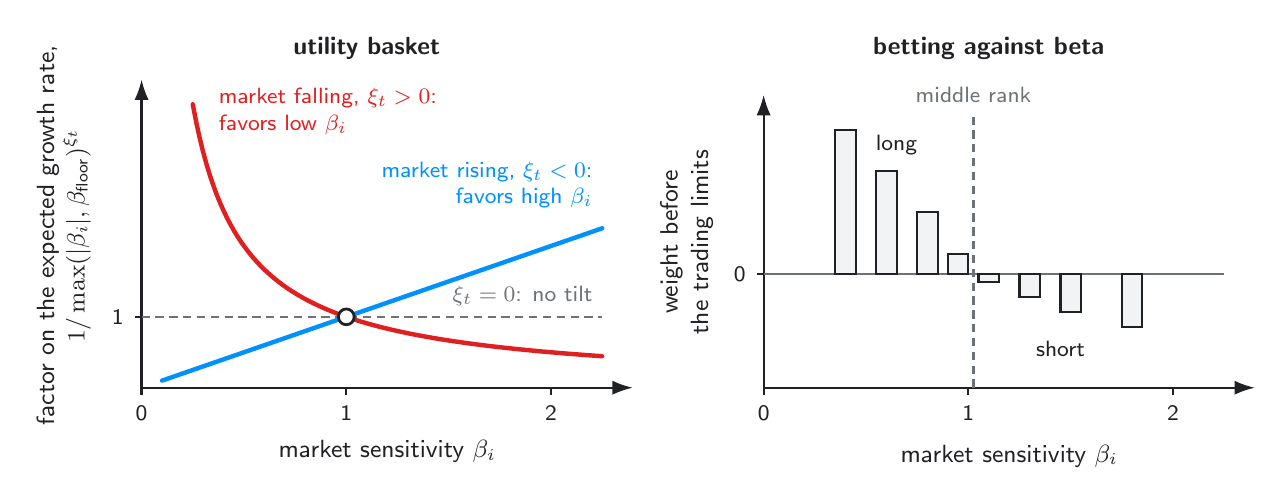
\begin{tikzpicture}[title/.style={font=\sffamily\small\bfseries, anchor=south}]
  % ---------------------------------------------------------------- the utility basket
  \begin{scope}[x=2.6cm, y=0.9cm]
    \node[title] at (1.1, 4.5) {utility basket};

    % axes
    \draw[axis] (0, 0) -- (2.4, 0);
    \draw[axis] (0, 0) -- (0, 4.35);
    \foreach \x in {0, 1, 2} {
      \draw[spine] (\x, 0) -- (\x, -0.1);
      \node[anchor=north, font=\sffamily\footnotesize] at (\x, -0.12) {\x};
    }
    \draw[spine] (0, 1) -- (-0.03, 1);
    \node[anchor=east, font=\sffamily\footnotesize] at (-0.04, 1) {1};
    \node[font=\sffamily\small, anchor=north] at (1.2, -0.6) {market sensitivity $\beta_{i}$};
    \node[font=\sffamily\small, rotate=90, anchor=south, align=center] at (-0.2, 2.15) {factor on the expected growth rate,\\$1/\max(|\beta_{i}|,\beta_{\text{floor}})^{\xi_{t}}$};

    % the three market states
    \draw[drop] (0, 1) -- (2.25, 1);
    \draw[curve, draw=gdred] plot[domain=0.25:2.25, samples=120] (\x, {1/\x});
    \draw[curve, draw=gdblue] (0.1, 0.1) -- (2.25, 2.25);
    \node[pt] at (1, 1) {};

    % labels
    \node[font=\sffamily\footnotesize, text=gdred, anchor=west, align=left] at (0.33, 3.9) {market falling, $\xi_{t}>0$:\\favors low $\beta_{i}$};
    \node[font=\sffamily\footnotesize, text=gdblue, anchor=south east, align=right] at (2.25, 2.4) {market rising, $\xi_{t}<0$:\\favors high $\beta_{i}$};
    \node[font=\sffamily\footnotesize, text=gdgray, anchor=south east] at (2.25, 1.02) {$\xi_{t}=0$: no tilt};
  \end{scope}

  % ---------------------------------------------------------------- betting against beta
  \begin{scope}[shift={(7.9, 1.44)}, x=2.6cm, y=2.4cm]
    \node[title] at (1.1, 1.0875) {betting against beta};

    % axes: the market sensitivity axis sits at the bottom, the zero weight line through the bars
    \draw[axis] (0, -0.6) -- (2.4, -0.6);
    \draw[axis] (0, -0.6) -- (0, 0.95);
    \foreach \x in {0, 1, 2} {
      \draw[spine] (\x, -0.6) -- (\x, -0.64);
      \node[anchor=north, font=\sffamily\footnotesize] at (\x, -0.645) {\x};
    }
    \draw[spine, draw=gdgray] (0, 0) -- (2.25, 0);
    \draw[spine] (0, 0) -- (-0.03, 0);
    \node[anchor=east, font=\sffamily\footnotesize] at (-0.04, 0) {0};
    \node[font=\sffamily\small, anchor=north] at (1.2, -0.85) {market sensitivity $\beta_{i}$};
    \node[font=\sffamily\small, rotate=90, anchor=south, align=center] at (-0.2, 0.17) {weight before\\the trading limits};

    % the middle rank splits the basket into the long and the short half
    \draw[drop] (1.025, -0.6) -- (1.025, 0.86);
    \node[note, anchor=south] at (1.025, 0.86) {middle rank};

    % the weights of weigh_bab for the eight made-up stocks
    \foreach \b/\w in {0.4/0.765, 0.6/0.5464, 0.8/0.3279, 0.95/0.1093, 1.1/-0.0398, 1.3/-0.1195, 1.5/-0.1992, 1.8/-0.2789} {
      \filldraw[fill=boxfill, draw=vnink, line width=0.8pt] (\b - 0.05, 0) rectangle (\b + 0.05, \w);
    }
    \node[font=\sffamily\footnotesize, anchor=south west] at (0.5, 0.58) {long};
    \node[font=\sffamily\footnotesize, anchor=north] at (1.45, -0.3) {short};
  \end{scope}
\end{tikzpicture}
\end{document}
